\documentclass[review]{elsarticle}

\usepackage{lineno,hyperref}
\usepackage[utf8]{inputenc}
\modulolinenumbers[5]

\journal{Renato Vimieiro}

%%%%%%%%%%%%%%%%%%%%%%%
%% Elsevier bibliography styles
%%%%%%%%%%%%%%%%%%%%%%%
%% To change the style, put a % in front of the second line of the current style and
%% remove the % from the second line of the style you would like to use.
%%%%%%%%%%%%%%%%%%%%%%%

%% Numbered
%\bibliographystyle{model1-num-names}

%% Numbered without titles
%\bibliographystyle{model1a-num-names}

%% Harvard
%\bibliographystyle{model2-names.bst}\biboptions{authoryear}

%% Vancouver numbered
%\usepackage{numcompress}\bibliographystyle{model3-num-names}

%% Vancouver name/year
%\usepackage{numcompress}\bibliographystyle{model4-names}\biboptions{authoryear}

%% APA style
%\bibliographystyle{model5-names}\biboptions{authoryear}

%% AMA style
%\usepackage{numcompress}\bibliographystyle{model6-num-names}

%% `Elsevier LaTeX' style
\bibliographystyle{elsarticle-num}
%%%%%%%%%%%%%%%%%%%%%%%

\begin{document}

\begin{frontmatter}

\title{Uma análise sistemática dos métodos avaliativos para classificação de filmes}

%% Group authors per affiliation:
\author{Gabriel D'Luca Souza Viana\fnref{gdsv}}
\author{Vitor Antônio de Lima Silva\fnref{vals}}
\address{Universidade Federal de Pernambuco – Centro de Informática
\linebreak Caixa Postal 7.851 – 50.732-970 – Recife, PE – Brasil
\linebreak gdsv@cin.ufpe.br, vals@cin.ufpe.br}

\fntext[gdsv]{Estudante de graduação do curso bacharelado em Sistemas de Informação}
\fntext[vals]{Estudante de graduação do curso bacharelado em Sistemas de Informação}

\begin{abstract}
Este documento foi elaborado com o objetivo de agregar uma série de informações referentes à nossa pesquisa, mais especificamente sobre os mecanismos que sumarizam os principais escores avaliativos do Metacritic. Com o auxílio de diversas ferramentas disponíveis para ciência dos dados, buscamos compreender as principais variáveis que regem e exercem influência nos principais critérios de avaliação do site – a exemplo do Metascore e do escore global dos usuários –, assim como suas inter-relações, como uma forma de melhor compreender e delinear uma visualização do cenário contemporâneo de resenhas de filmes. 
\end{abstract}

\end{frontmatter}

\linenumbers

\section{Introdução}

Um dos mais tradicionais websites para agregação de críticas, o Metacritic sintetiza avaliações de publicações reputadas sobre um determinado filme, álbum, jogo eletrônico ou série de televisão. Desde 1999, o site é responsável por realizar uma agregação de notas e converter para uma escala de 0 à 100 pontos, reunindo a nota atribuída por cada crítico em uma única avaliação ponderada global, denominada Metascore. Este relatório tem como objetivo reunir as análises e estudos que conduzimos no Metacritic, a fim de verificar o cenário atual das resenhas dos filmes baseando-se em avaliações do The New York Times. 

\section{Método}

Objetivamos conduzir análises no popular website para agregação de críticas, o Metacritic. Para a concretização de nosso estudo, utilizamos a linguagem de programação Python 3 ao decorrer de diversas etapas — desde a coleta até a análise. A partir desta, desenvolvemos \textit{scripts} para realizar a coleta dos filmes avaliados pelo The New York Times conforme o site, integrando os dados obtidos com os dados de detalhes de cada filme. Em seguida, realizamos etapas de pré-processamento para que pudéssemos transformar os dados de forma que estes se tornassem compátiveis com as análises que pretendíamos realizar.

Isso feito, o próximo passo fora utilizar de diversas bibliotecas da linguagem de programação que possibilitassem a realização de nossas análises. Através da elaboração de visualizações, buscamos compreender os critérios que influenciam as diferentes avaliações do site — a exemplo do escore global dos críticos (denominado Metascore) e dos usuários — em um nível macro, mas sem perder de vista as interrelações e correspondências existentes a nível micro.

\section{Coleta}

Inicialmente, realizamos a análise do código-fonte das páginas que desejávamos extrair — mais especificamente, da página da publicação do The New York Times (\url{http://www.metacritic.com/publication/the-new-york-times}) e da página de detalhes de cada filmes (\url{http://www.metacritic.com/movie/call-me-by-your-name/details}). Isso feito, desenvolvemos \textit{scripts} que automatizassem estas coletas. Para isso, utilizamos as bibliotecas \textit{Requests} e \textit{BeautifulSoup}, de Python, que foram essenciais para este processo. Modelamos o dados coletados no formato de um DataFrame, conforme utilizado pela biblioteca \textit{Pandas}, e salvamos os conteúdos extraídos em arquivos no formato CSV.

\section{Pré-processamento}

Adiante, realizamos a criação de um \textit{notebook} a partir da ferramenta \textit{Jupyter Notebook}, utilizada para a criação de um documento que possibilitasse o acompanhamento de cada etapa realizada pela equipe. Inicialmente, realizamos a leitura dos arquivos CSVs gerados durante a coleta e partimos para a etapa de pré-processamento dos dados. Removemos dados que foram perdidos durante a extração das páginas, convertemos cada dado para seu tipo de atributo correspondente e, por conseguinte, discretizamos alguns dados em intervalos que corroborassem com a execução da análise. Como extraímos um grande conjunto de dados, a alternativa que escolhemos para o tratamento dos dados ausentes fora simplesmente ignorá-los durante a análise, visto que isso não impactaria tanto nossas observações. Por fim, realizamos a integração dos dados em um único arquivo CSV a ser utilizado para a análise.

\section{Análise exploratória}

Finalmente, partimos para a análise explorátoria. Iniciamos nossa pesquisa buscando responder as seguintes perguntas: “quão forte é a influência no Metascore por parte da nota atribuída pelos críticos do The New York Times?”; “dentre os críticos do The New York Times, quais atribuem um maior número de notas positivas, mistas e negativas em suas avaliações?”.

\begin{figure}[!ht]
  \centering
  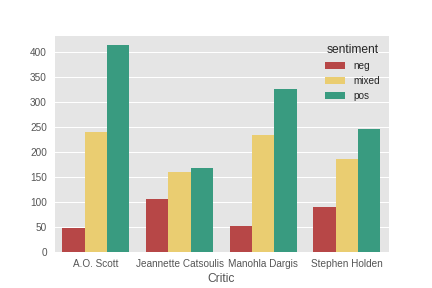
\includegraphics[width=288px]{../observations/sentiment-per-critics.png}
  \caption{Distribuição das avaliações dos quatro principais críticos do The New York Times.}
  \label{fig:sentPerCritic}
\end{figure}

No geral, é possível identificar que nem todos os críticos possuem a mesma distribuição de notas internamente. Tratando-se do crítico A.O Scott, por exemplo, podemos verificar que há a atribução de uma quantidade substancial de avaliações positivas em relação aos demais. Similarmente, também é possível verificar que críticos como a Jeannette Catsoulis apresentam um maior balanceamento de notas, com menos da metade de avaliações positivas em relação ao A.O Scott e pouco mais do dobro de avaliações negativas em relação ao mesmo, conforme podemos verificar na Figura \ref{fig:sentPerCritic}. 

Ainda assim, é preciso levar em consideração, também, que uma influência negativa do Metascore não significa que esta é uma relação desfavorável — pelo contrário, se um crítico atribui mais notas negativas em suas avaliações, uma redução concomitante do Metascore significa que este ainda é ativamente influente.

\begin{table}[!h]
  \centering
  \includegraphics[width=\linewidth]{./images/table-critics-per-sent.png}
  \caption{Distribuição das avaliações dos quatro principais críticos do The New York Times por sentimento.}
  \label{fig:sentPerCriticTable}
\end{table}

Em uma análise mais detalhada, é possível verificar a quantificação desta influência varia conforme o sentimento por crítico, conforme pode-se conferir na Tabela \ref{fig:sentPerCriticTable}. Interpretam-se os resultados como a seguir: considerando as resenhas mistas do crítico A.O Scott como base, é possível ver que este costuma atribuir notas mistas maiores em suas resenhas do que em comparação à outros críticos, enquanto Stephen Holden costuma atribuir notas mistas menores que os demais. Quanto às avaliações negativas, estima-se que Jeannette Catsoulis atribua as menores notas. Já entre o polo de reviews positivas, Jeannette atribui as mais baixas, enquanto A.O Scott introduz, novamente, notas superiores em relação aos demais. 

\begin{figure}[!h]
  \centering
  \includegraphics[scale=0.7]{./images/score-infl-per-genre-1.png}
  \caption{Influência da categorização por gênero no Metascore.}
  \label{fig:metascoreInflPerGenre}
\end{figure}

Seguimos para a próxima pergunta: “quais gêneros constumam ser atribuidos a maiores e menores índices de aclamação [dos críticos]?”. Conforme a Figura \ref{fig:metascoreInflPerGenre}, é possível verificar que, em uma escala de primeiro nível e estimando-se um valor padrão para o Metascore, os documentários, filmes de animação e de drama estão associados a Metascores maiores (e consequentemente, a maiores índices de aclamação no site), enquanto filmes de ação e filmes de terror se encontram associados a Metascores abaixo do que o habitual. 

Por conseguinte, para possibilitar uma resposta mais concreta, elaboramos, ainda, \textit{boxplots} para verificar a distribuição interna do Metascore e dos escores atribuídos ao The New York Times nos cinco principais gêneros, conforme pode ser verificado nas Figuras \ref{fig:metascoreDistPerGenreOne} e \ref{fig:metascoreDistPerGenreTwo}, que se encontram dispostas na página logo abaixo.

\begin{figure}[!h]
  \centering
  \includegraphics[scale=0.7]{./images/score-dist-per-genre-1.png}
  \caption{Distribuição do Metascore por gênero.}
  \label{fig:metascoreDistPerGenreOne}
\end{figure}

\begin{figure}[!h]
  \centering
  \includegraphics[scale=0.7]{./images/score-dist-per-genre-2.png}
  \caption{Distribuição das notas do The New York Times por gênero.}
  \label{fig:metascoreDistPerGenreTwo}
\end{figure}

Partiremos, agora, para outra pergunta que buscamos responder: “o quanto o Metascore influencia no escore global dos usuários?”. Para esta pergunta, também buscamos levar em consideração o fator das décadas de lançamento do filme, conforme podemos verificar na Figura \ref{fig:metaInflInUser}, onde a imagem da esquerda corresponde aos anos 2000, e a da direita aos anos 2010.

\begin{figure}[!h]
  \centering
  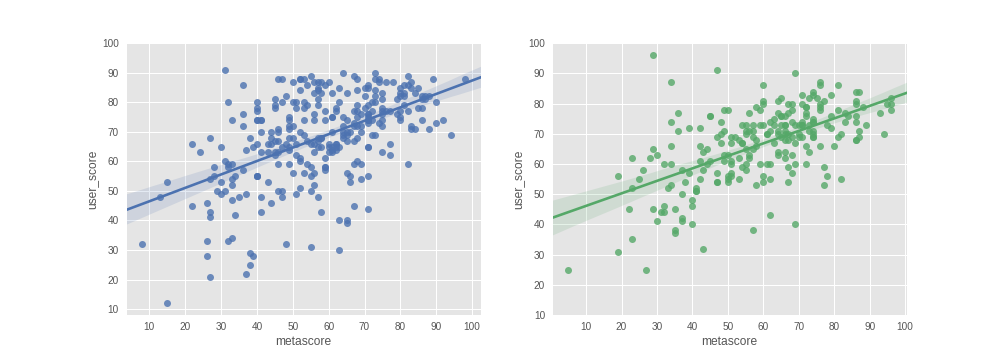
\includegraphics[width=\linewidth]{../observations/metascore-infl-comparison.png}
  \caption{Influência do Metascore no escore global dos usuários.}
  \label{fig:metaInflInUser}
\end{figure}

É possível ver que a influência do Metascore sobre o escore global dos usuários aumentou um pouco em relação à última década, apesar de ambas se demonstrarem igualmente pertinentes de que esta influência realmente existe e é significativa, onde atualmente há um aumento de aproximadamente 7 pontos no escore dos usuários a cada 20 pontos adicionados no Metascore.

Para concluírmos, a última pergunta que buscamos responder foi: “existe alguma associação entre as demais características do filme e o Metascore?”. Sumarizando o que encontramos em nossas análises, conforme podemos verificar na Figura \ref{fig:langInflInMetascore} e considerando os filmes em inglês como padrão, é possível ver que os filmes em outros idiomas tendem a possuir escores superiores. Os filmes japoneses possuem a maior influência no Metascore com sua categorização, seguidos pelos filmes alemães, franceses, logo após, espanhóis. Assim sendo, é possível verificar que os idiomas também se apresentam fatores consideráveis e de influência.

\begin{figure}[ht]
  \centering
  \includegraphics[scale=0.7]{./images/score-infl-per-lang-1.png}
  \caption{Influência da categorização por idioma no Metascore.}
  \label{fig:langInflInMetascore}
\end{figure}

Ao contrário do que esperávamos, conforme pode ser visto na Tabela \ref{fig:directorsInflInMetascore}, ao conduzirmos uma análise mais cuidadosa com os principais diretores, é possível ver que estes não possuem uma influência propriamente dita, visto que o p-value apresentado por estes é alto — o que indica que não podemos rejeitar a hipótese de que estes não são influentes. Além disso, é possível verificar que o alto p-value da estatística F, mostrado logo após a tabela, permite-nos concluir que, com a inclusão dos diretores como variavéis, não é possível rejeitar a hipótese nula de que não estamos melhorando a qualidade de nosso modelo.

\begin{table}[h]
  \centering
  \includegraphics[scale=0.7]{./images/table-directors-infl.png}
  \caption{Influência dos diretores no Metascore.}
  \label{fig:directorsInflInMetascore}
\end{table}

Finalizaremos aqui a seção de análises como uma forma de manter o balaceamento de conteúdo neste relatório. Não obstante, foram conduzidas diversas análises adicionais visando analisar as inter-relações presentes nos métodos avaliativos do site e estas podem ser conferidas na íntegra nos \textit{notebooks} disponibilizados no repositório do GitHub da nossa pesquisa (\url{https://github.com/if1015-datascience-ufpe/2017-2-projeto-metascience}).

\section{Classificação de texto}

Por fim, fizemos modelos de classificação de texto para tentar predizer o sentimento do autor de uma resenha a respeito de um filme, dado o seu texto. Esses classificadores são treinados associando uma considerável quantidade de palavras aos seus respectivos sentimentos. Ao fazer essa associação, os algoritmos podem analisar cada palavra de uma resenha e, usando o que aprendeu com os dados previamente passados para ele, atribuí-la a uma classe positiva, negativa e neutra.  

A fim de otimizar os modelos, as resenhas passaram por uma série de tratamentos para maximizar a quantidade de informação extraída de cada uma das palavras no seu texto. Para isso, utilizamos um tokenizador inteligente da biblioteca NLTK (do inglês, \textit{Natural Language Toolkit}). Após a tokenização, cada uma das palavras é convertida para letras minúsculas e passa pelo processo de lematização, que consiste em deflexionar as palavras, buscando seu lema. Em seguida, como forma de reforço, as palavras são tratadas por \textit{stemming} para minimizar a quantidade de palavras não lematizadas corretamente. Por fim, as palavras recebem suas respectivas classes e estão prontas para serem passadas para os classificadores.

Utilizamos 70\% (cerca de 8400) dos dados como conjunto de treino, enquanto os outros 30\% (cerca de 4000) foram utilizados para testar a acurácia de cada um dos classificadores. A partir disso, foram treinados 7 modelos de classificação de texto, entre eles:

\begin{itemize}
	\item{Naive Bayes Classifier}
	\item{Multinomial Naive Bayes Classifier}
	\item{Linear Regression Classifier}
	\item{Stochastic Gradient Descent Classifier}
	\item{Support Vector Classifier}
	\item{Linear Support Vector Classifier}
	\item{Nu Support Vector Classifier}
\end{itemize}

Ao verificar a acurácia média dos modelos apresentados acima, obtivemos uma média de apenas 55.30\%. Verificando a divergência entre os resultados dos classificadores, decidimos criar um novo classificador: o classificador por voto. Este funcionaria como um detector de moda entre os resultados dos outros classificadores, classificando a resenha com a classe mais comum entre eles. A acurácia desse classificador por voto também ficou próximo da média, sendo, geralmente, o segundo melhor classificador, perdendo apenas para o Multinomial Naive Bayes, que mostrou ser o melhor em todos os casos e acertando cerca de 60\% das predições. Em seguida, foram feitas investigações com três diferentes conjuntos de testes a fim de encontrar \textit{bias} nos classificadores, o primeiro conjunto foi composto por resenhas exclusivamente negativas, enquanto o segundo por resenhas exclusivamente positivas e o terceiro, neutras. 

Descobrimos, a partir disso, que o Support Vector Classifier classificava todas as resenhas como positivas, pois apresentou acurácia de 100\% para o conjunto de teste exclusivamente positivos e 0\% para os conjuntos neutros e negativos, o que nos levou a descartá-lo. Não obstante, ao fazermos algumas predições com frases contendo palavras significativas, todos os modelos se mostraram bastante razoáveis, classificando como positiva a frase “I love this movie!”, enquanto a frase “Even though I think it's average, my wife loves it!” fora classificada como positiva ou neutra e, por fim, a frase “What a terrible movie, I was bored the whole time!”, como negativa.  

\section{Considerações finais}

A possibilidade da realização de nossas análises nos permitiu uma melhor compreensão dos critérios de influência entre os diversos classificadores avaliativos do Metacritic. Por sua vez, a elaboração de \textit{notebooks} e utilização de diversas bibliotecas que conduzissem nosso estudo demonstraram a utilidade e a importância do domínio destas ferramentas no campo de ciência dos dados, bem como a do conhecimento da linguagem de programação Python. 

Por conseguinte, as diversas visualizações mostradas ao decorrer deste relatório corroboram com o processo de delineamento da influência de diversos fatores nos escores. A partir das análises realizadas, fora possível identificar que essas avaliações, apesar de se apresentarem correlatas em um primeiro momento, divergem internamente conforme a consideração de atributos diversos. Tivemos a oportunidade de ter hipóteses atestadas, contestadas, e visualizar o surgimento de novas ao decorrer de nossas análises. 

Uma vez que conseguimos realizar um mapeamento geral do panorama dos critérios avaliativos do site, há a possibilidade de condução de estudos posteriores que busquem priorizar a estimação destes, utilizando os diversos critérios de influência que encontramos para o cálculo de um peso único para a publicação — de forma similar ao site (\url{http://www.metacritic.com/about-metascores}). Considerando uma equipe maior e um período de médio a longo prazo, poderiam ser consideradas, ainda, as demais publicações neste processo, buscando estimar e realizar normalizações para cada escore de modo a tornar as predições mais assertivas, mas sem perder de vista a ótica inter-relacional e sistemática necessária para sua concretização.

\end{document}
